% Chapter 2
\chapter{Social Accounting Matrix for Scotland}
\label{Chapter2}

\section{Introduction} 
\label{sec:2.1}

This chapter outlines the methodology and computations used to construct the 2009 Social Accounting Matrix (SAM) for Scotland. A SAM can be described as a static image (a snapshot) of the flow of goods, services and factors, and the concurrent flow of funds between agents in an economic system for a given time-period \shortcite{Hosoe2010a}. Essentially, the computed SAM extends the Scottish Input Output (IO) tables by incorporating an Income and Expenditure (IncExp) account. Thus, the IncExp account contains information on institutional accounts that is not recorded within the IO tables. Therefore the SAM can be used to analyse social and economic policy in a more comprehensive way. The main benefits and structure of a SAM are outlined in the first sections.  Next, the computed IncExp account and the 2009 Scottish IO tables are combined to complete the 2009 SAM for Scotland. In the last section, the methodology required to compute the IncExp account is described in detail.

%%%%%%%%%%%%%%%%%%%%%%%%%%%%%%%%%%%%%%%%%%%%%%%%%%%%%%%%%%
%SECTION
%%%%%%%%%%%%%%%%%%%%%%%%%%%%%%%%%%%%%%%%%%%%%%%%%%%%%%%%%%
\newpage
\section{Social Accounting Matrices} 
\label{sec:2.2}

The SAM can be considered as an extension to an IO table which not only records macroeconomic-aggregates but also the distribution and redistribution of income. The focus of a SAM therefore lies in recording interrelationships at the meso-level with emphasis on distributive aspects \cite{Keuning1988a}. A SAM can therefore be described as being concerned with the systematic organisation of information about the economic and social structure of a country, region, city or other unit, in a particular time period - usually a year \cite{King1981a}.

\bigskip

In contrast to IO tables, the SAM records flows from producing sectors to factors of production and then on to institutional accounts and finally back to demand for goods \cite{Adelman1986a}. As such, a SAM is different from an IO table as it contains complete information on institutional accounts (i.e. households, government and corporations), instead of solely tracing income and expenditure flows of activities and commodities \shortcite{Breisinger2010a}. The main features of a SAM can be divided into three sections \cite{Round2003a}:   

\bigskip

First, the SAM is a square matrix where the rows represent the flow of goods$/$factors in money terms, whilst the columns represent the flow of payments. The SAM records the expenditures down the columns and the receipts along the rows. The row sums in the SAM show the total receipts and the column sums show the total payments of funds. Importantly, each row sum must equal its corresponding column sum. That is, the total revenue must equal total expenditure in each account \shortcite{Hosoe2010a}. Each cell in the SAM represents a flow of funds from a column account to a row account, thereby documenting the interconnections between these accounts in an explicit way and identifying the source and use of all transactions. 

\bigskip

Second, the SAM is considered to be comprehensive as it shows economic activity in terms of consumption, production, accumulation and distribution (although not necessarily in equivalent detail). 

\bigskip

Third, the SAM is considered to be flexible in the degree of disaggregation, whilst at the same time following a basic accounting framework \shortcite{Breisinger2010a}. The degree of disaggregation generally depends on the motivation behind constructing the SAM (e.g. depending on the location of the initial shock and the outcome variables) and more restrictively, the availability of data \cite{Round2003a}. 

\bigskip

The benefits arising from computing a SAM are multifold. The additional information contained in the SAM, compared to IO tables, can be used to extend and improve the multiplier modelling capacity to include the behaviour of the non-production part of the economy. In particular, the link between activity and changes in household income should improve the Type II multiplier. 

\newpage

Moreover, in contrast to national accounts, the SAM can incorporate a highly disaggregated social breakdown. This is particularly important as a large number of economic interactions happen within the household sector. That is, income from labour and the household sector can be further broken down to analyse distributional effects of policy more accurately \cite{Stuttard2003b}. 

\bigskip

An important side-effect of the compilation process of a SAM is that data gaps and inconsistencies can be identified. This information can be used to improve and extend survey methodologies, definitions and classifications and overall compatibility of data sources \cite{Keuning1988a}. 

\bigskip

The main utility, however, of a SAM is that it provides a comprehensive and consistent record of the interrelationships of an economy at the level of individual production sectors, factors, and institutions. Thereby, the SAM makes available an internally consistent statistical foundation, or benchmark, for the creation of plausible economic models (e.g. Computable General Equilibrium models) which simulate changes to the economy \cite{Reinert1997a}.     

%%%%%%%%%%%%%%%%%%%%%%%%%%%%%%%%%%%%%%%%%%%%%%%%%%%%%%%%%%
%SECTION
%%%%%%%%%%%%%%%%%%%%%%%%%%%%%%%%%%%%%%%%%%%%%%%%%%%%%%%%%%
\newpage
\section{Social Accounting Matrix for Scotland} 
\label{sec:2.3}

The main components of the SAM are the latest Scottish IO tables for Scotland \cite{ScottishGovernment2013a} and the IncExp account. More precisely, the 2009 Industry by Industry (IxI) table for Scotland at basic prices is used. The IxI table is a symmetric IO table with industries (104 industries at SIC07) as the dimension of both rows and columns. Thereby the IxI table records the destination of manufacturing industry outputs. The data on industry linkages can be used to analyse knock-on effects throughout the Scottish economy of a change of final demand \cite{ScottishGovernment2011a}. 

\bigskip

Table \ref{tab:2.3.1} depicts the final SAM that is derived by combining the IxI table and the IncExp account. For illustration several accounts have been aggregated. For example, the 104 industries contained in the SAM are aggregated to one industry (Activities). Thus, it must be emphasises that, for modelling purposes, a more detailed SAM is used.   

\bigskip

As outlined previously, the aggregate 2009 SAM or Scotland is a square matrix with 7 column and 7 row accounts. The rows represent the flow of goods$/$factors in money terms, whilst the columns represent the flow of payments. The SAM records the expenditures down the columns and the receipts along the rows. The row sums in the SAM show the total receipts and the column sums show the total payments of funds. Each row sum equals its corresponding column sum. That is, the total revenue is equal total expenditure in each account. Each cell in the SAM represents a flow of funds from a column account to a row account, thereby documenting the interconnections between these accounts in an explicit way and identifying the source and use of all transactions. 

\bigskip

\begin{table}[H] \caption{Aggregate 2009 SAM for Scotland (in \textsterling million)}
\bigskip \begin{scriptsize} \begin{centering} \begin{doublespacing}
    \begin{tabular}{lrrrrrrrr}
          \toprule
          & \begin{sideways}1. Activities (IOC1-104)\end{sideways} & \begin{sideways}2. Households\end{sideways} & \begin{sideways}3. Corporate\end{sideways} & \begin{sideways}4. Government\end{sideways} & \begin{sideways}5. Capital\end{sideways} & \begin{sideways}6. Employment Income\end{sideways} & \begin{sideways}7. Exports to RUK + ROW\end{sideways} & \begin{sideways}Total (Receipts)\end{sideways} \bigstrut\\
    \hline
    1. Activities (IOC1-104) & 63,607 & 49,802 & -     & 29,486 & 13,981 & -     & 54,045 & 210,920 \\
    2. Households & -     & -     & \textbf{15,104} & \textbf{25,124} & -     & 63,561 & \textbf{4,088} & 107,877 \\
    3. Corporate & -     & \textbf{6,931} & -     & \textbf{34,647} & -     & -     & \textbf{11,928} & 53,507 \\
    4. Government & 43,221 & \textbf{27,947} & \textbf{5,248} & \textbf{16,861} & 1,495 & -     & \textbf{20,363} & 115,136 \\
    5. Capital & -     & \textbf{5,070} & \textbf{24,826} & \textbf{119}   & -     & -     & \textbf{-10,086} & 19,930 \\
    6. Employment Income & 63,561 & -     & -     & -     & -     & -     & -     & 63,561 \\
    7. Imports from RUK + ROW & 40,532 & \textbf{18,126} & \textbf{8,328} & \textbf{8,898} & \textbf{4,455} & -     & 10,470 & 90,808 \\
\bottomrule 
\end{tabular}%  
\bigskip \begin{flushright} Cells derived from the IncExp Account are \textbf{highlighted}. Remaining stem directly from the 2009 IxI table \cite{ScottishGovernment2013a}.\end{flushright} \label{tab:2.3.1} 
\end{doublespacing} \end{centering} \end{scriptsize} \end{table} \bigskip

The first row of the SAM, for example, can be read as follows: raw material purchases of goods within Scotland (\textsterling63,607m), Household consumption expenditure on goods$/$services (\textsterling49,802m), Government current expenditure (\textsterling29,486m), investment expenditure on Scottish goods (\textsterling13,981m), exports to RUK + ROW (\textsterling54,045m) and the total of \textsterling210,920m represents total aggregate demand of gross outputs.

\bigskip 

Extending the IO table by incorporating the IncExp accounts yields a SAM with the following entries (the * indicated that entries, with the exception of the IncExp extension, were directly taken from the IO table):

\bigskip

\begin{itemize}
    \item Activities are directly taken from the IO table and contains the 104 industries at SIC07. Activities show the destination of manufacturing industry outputs, including manufacturing products or other secondary products.
    \item Households are directly taken from the IO table* and is the sum of the Household account and the Non-Profit Institutions Serving Households (NPISHs) account in the IO table.
    \item Corporate is solely derived within the IncExp account, thereby providing a more complete record of the institutional account. 
    \item Government is directly taken from the IO table* and is the sum of the Central and Local Government accounts in the IO table.
    \item Capital is directly taken from the IO table* from Gross fixed capital formation (GFCF).
    \item Employment income is taken directly from the IO table*.
    \item Exports$/$imports to and from RUK$/$ROW (including good $/$ services and transfers) are directly taken from the IO table* RUK and ROW exports$/$imports entry.
\end{itemize}

\bigskip

Importantly, constructing the SAM by extending IO tables by means of an IncExp account does not require any rebalancing (e.g. total receipts per account match total expenditures). That is, the IO table is fully incorporated without the need of changing any entries thereof. All cells that were added to the IO table to compute the SAM are balanced within the IncExp account so that total revenue equal total expenditure in each account. This approach incorporates the IO tables at face value, assuming that the data therein are the best possible estimates of Scottish data. Each account in the Scottish SAM is balanced by their corresponding account. So for example, Government expenditures (\textsterling115,136m) are balanced by Government receipts (\textsterling115,136m). 

\bigskip

It must be emphasised again that the SAM is meant to fit around the existing IO tables and other national statistics. Data necessary for the construction of the SAM that are not contained within the IO table are derived by computing an IncExp account. This account records income and expenditure of households, corporations, government, capital and the external sector in detail. The construction of the IncExp account is outlined in the following section.

%%%%%%%%%%%%%%%%%%%%%%%%%%%%%%%%%%%%%%%%%%%%%%%%%%%%%%%%%%
%SECTION
%%%%%%%%%%%%%%%%%%%%%%%%%%%%%%%%%%%%%%%%%%%%%%%%%%%%%%%%%%
\newpage
\section{The Income and Expenditure Accounts for 2009}
\label{sec:2.4}

The Income and Expenditure Accounts provide a details on the flow of funds for the main three local transactors (Households, Corporations and Government) as well as for the Capital and External Accounts. The Accounts are compiled using publicly available data, including both UK and Scottish Government data as well as figures from the 2009 IO Tables for Scotland. The IncExp Accounts are internally consistent, which ensures that the SAM is automatically balanced. The above section outlined the role that the IncExp Accounts have in extending the IO Tables into a SAM for Scotland. This section provides an overview of how the IncExp Accounts are constructed and the following section gives a detailed breakdown of how each entry in the Accounts is calculated. First in this section, the layout of the Accounts is presented. Second, the data calculation and internal balancing is discussed. Third, the data sources used for the Accounts are  


\subsection{Layout}
\label{sec:2.4.1}

The IncExp Accounts (see Table \ref{tab:2.4.1}) are divided into five different sectors (Households, Corporations, Government, Capital and External) and they also give the Scottish Trade and External Balance with both RUK and ROW. Each of those sectors is divided further into an Income and an Expenditure part, hence the name for these Accounts. Each cell can be identified either through the name, e.g. Corporations > Income > Profit Income (OVA) or through the equivalent number code, 19 in this case. The latter method is used when cross-referencing in the detailed breakdown of the cells in the Methodology section (\ref{sec:2.5}).Every sector has a Total Income and a Total Expenditure Figure, which is a summation of the entries in each section (highlighted in bold). The Household and Government sector have additional Control Totals from external sources and therefore they are presented with two Totals. The Primary Sectors (Household, Corporations and Government) have a similar cell breakdown with Income/Payments to the other Primary Sectors as well as External Transfer payments making up the biggest share of entries. Additionally, all Primary Sectors have a Profit Income (OVA) entry and a Payments to Capital entry on the Income and on the Expenditure side, respectively. Cells with one star following the numerical entry refer to Balancing Items and those with two stars refer to Corresponding Figures. A detailed discussion of those entries can be found in Calculation Overview and Internal Balancing (\ref{sec:2.4.2}).


% % % % % % % % % % % % % % % % % % % % % % % % % % % % % % % % %
% % % % % % THE INCOME AND EXPENDITURE ACCOUNTS TABLE % % % % % %
% % % % % % % % % % % % % % % % % % % % % % % % % % % % % % % % %


\begin{table}[H] \caption{Income-Expenditure Accounts for Scotland (in \textsterling million)}
\bigskip \begin{scriptsize} \begin{centering} \begin{spacing}{1.2}
    \begin{tabular}{lrllrl}
          \toprule
    \textbf{HOUSEHOLDS} \bigstrut\\
    \hline  
\bigstrut[t]    1. \textbf{Income} & \textbf{107877} & & 10. \textbf{Expenditure} & \textbf{107877} & \\
    2. Income from Employment & 63561  &   & 11. IO Expenditure & 74138 & \\
    3. Profit Income (OVA) & 5289 & & 12. Payments to Corporations & 6931 &* \\
    4. Income from Corporations & 15104 & & 13. Payments to Government & 21379 & \\
    5. Income from Government & 19835 & & 14. Transfers to ROW & 119 & \\
    6. Transfers from RUK & 1852 & & 15. Transfers to RUK & 238 & \\
    7. Transfers from ROW & 2237 & & 16. Payments to Capital (Savings) & 5070 &\\
    8. \textbf{Total Household Income} & \textbf{107877} & & 17. \textbf{Total Expenditure} & \textbf{107877} & \\
    9. \textbf{Mixed and Prop Income Unalloc.} & 0 & \bigstrut[b]\\
    \hline
\bigstrut[t]    \textbf{CORPORATIONS} \bigstrut\\
    \hline
\bigstrut[t] 18. \textbf{Income} & \textbf{53507}  &   & 24. \textbf{Expenditure} & \textbf{53507} & \\
       19. Profit Income (OVA) & 29456 & & 25. Payments to Households & 15104 &** \\
       20. Income from Households & 6931 &** & 26. Payments to Government & 5248 & \\
       21. Income from Government & 5191 &** & 27. Transfers to RUK & 3768 & \\
       22. Income from RUK & 5964 & & 28. Transfers to ROW & 4560 & \\
       23. Income from ROW & 5964 & & 29. Payments to Capital (Savings) & 24826 &* \\
    \hline
    \textbf{GOVERNMENT} \bigstrut\\
    \hline
\bigstrut[t]       30. \textbf{Income} & \textbf{63530}  &   & 37. \textbf{Expenditure} & \textbf{63530} & \\
       31. Profit Income (OVA) & 3697 & & 38. IO Expenditure & 30017 & * \\
       32. Net Commodity Taxes & 13165 & & 39. Payments to Corporations & 5191 &* \\
       33. Income from Households & 21379 &** & 40. Payments to Households & 19835 &** \\
       34. Income from Corporations & 5248 &** & 41. Transfers to RUK & 8368 & \\
       35. Income from RUK & 20041 &* & 42. Payments to Capital (Savings) & 119 & \\
       36. \textbf{Total Govt Inc Balancing Total} & \textbf{63530} &** & 43. \textbf{Total Govt Exp Balancing Total} & \textbf{63530} &  \\ 
    \hline
    \textbf{CAPITAL} \bigstrut\\
    \hline
\bigstrut[t]       44. \textbf{Income} & \textbf{19930}  &   & 49. \textbf{Expenditure} & \textbf{19930} & \\
       45. Households & 5070 &** & 50. IO Expenditure & 19930 &  \\
       46. Corporations & 24826 &** &  \\
       47. Government & 119 &** &  \\
       48. RUK/ROW & -10086 &** &  \\ 
    \hline
    \textbf{EXTERNAL} \bigstrut\\
    \hline
\bigstrut[t]  51. RUK Income from Scotland & 67133  &   & 58. RUK Expenditure in Scotland & 70595 & \\
       52. Goods \& Services & 54759 & & 59. Goods \& Services & 42739 & \\
       53. Transfers & 12374 & & 60. Transfers & 27857 & \\
       54. RUK Income from Scotland & 23676 & & 61. ROW Expenditure in Scotland & 27378 & \\
       55. Goods \& Services & 18997 & & 62. Goods \& Services & 19178 & \\
       56. Transfers & 4679 & & 63. Transfers & 8201 & \\
       & & & 64. Tourist Expenditure in Scotland & 2921 & \\
       57. \textbf{Total Income} & \textbf{90808} & & 65. \textbf{Total Expenditure} & \textbf{100894} &  \\  
        & & & 66. Surplus/Deficit &-10086 & \\   
    \hline
    \textbf{G\&S TRADE BALANCE} \bigstrut\\
    \hline
\bigstrut[t] \quad \enspace \thinspace Scotland with RUK and ROW & &   & \quad \enspace \thinspace Total Balance of Payments & & \\
       67. RUK & -12020 & & 69. RUK & 5215 &  \\
       68. ROW & 181 & & 70. ROW & 4871 & \\
       & & & 71. Total Balance of Payments & 10086 & \\  
    \hline    
    \textbf{EXTERNAL BALANCE} \bigstrut\\
    \hline
\bigstrut[t]   72. Income from Employment & -3462 & & & & \\
       73. Profit Income (OVA) & -3703 & & & &  \\
       74. Income from Corporations & -2921 & & & & \\
       75. Income from Government & -10086 & & & & \\ 
    \hline
    \hline    
\qquad \qquad \qquad Balancing Item: *   & & & Row Entries (Element determines Column)  \\ 
\qquad \qquad \qquad Corresponding Figure: ** & & & Row Entries (Element determines Column)  \bigstrut\\       
          \hline            
    \bottomrule
\end{tabular}%  
\bigskip \begin{flushright}\end{flushright} \label{tab:2.4.1}
\end{spacing} \end{centering}  \end{scriptsize} \end{table}


\subsection{Calculation Overview and Internal Balancing}
\label{sec:2.4.2}

Most of the figures in the Accounts are calculated using either figures from the IO Tables or external sources. The references for each calculation are both in the Methodology Section  (\ref{sec:2.5}) as well as within the SAM file. Most governmental data is issued in the financial year format, i.e. April of year one until end of March of year 2. In order to get data for the calendar year 2009, which is also the format of the IO Tables, a one-quarter share of the year one data is taken and a three-quarter share of year two (1/4*2008/09 + 3/4*2009/10). Using the updated 2006 SAM, the data sources for each IncExp Account entry are updated and when possible more accurate sources/figures are used in the calculation of the 2009 Accounts.
Some cells, however, are not calculated using the above-mentioned sources. First, some cells are Balancing Items, denoted with one star (see Table \ref{tab:2.4.1}). These entries are derived by taking the Totals of the relevant account and deducting the sum of all other entries, but the one marked as a Balancing Item. The reason for this methodology is two-fold. On the one hand, in order to balance the Total Income and the Total Expenditure of the Primary Sectors, at least one entry needs to absorb any deviation in the balance between income and expenditure. On the other hand, for some cells the data availability or quality is simply not there and thus those entries with the least robust data are chosen to be Balancing Items. The Balancing Items further ensure the internal consistency of the IncExp Accounts and therefore the SAM balances automatically once the IO Tables are extending through these Accounts. Second, there are cells denoted with two stars and these are the Corresponding Figures. Due to the assumption of the Circular Flow of the Economy, where the income that a receives from b is equal to the payment that b makes to a, some entries are equal to the figures derived for other cells. For example, the Payments to Government made by Corporations (cell 26) is equal to the Income from Corporations received by the Government. Further, all Income entries for the Capital Accounts are Corresponding Figures, as these are equal to the Payments to Capital entries by each of the Primary Sector as well as the net External balance (cell 66). 


\subsection{Data}
\label{sec:2.4.3}

The data used in the construction of the IncExp Accounts is all taken from either UK or Scottish Government sources and is publicly available. Figure \ref{fig:2.4.1} shows how much data is derived from the main data sources. For this, each component of the IncExp cells is deconstructed. For example, some cells use one figure from the IO Tables, one from GERS (Government Expenditure and Revenue Scotland) and one from the HM Treasury. This would give three separate sources which would be counted as individual entries and then the total of those entries' is used to calculate the shares allocated to each source of data origin. Note, that when data is given in financial year format, there are technically two entries from that source, which is then transformed into a calendar year entry, as outlined above. However, this is then taken as a single entry for the calculation of the shares here, as it would otherwise skew the percentages. As Figure \ref{fig:2.4.1} shows the three biggest sources for data used in the IncExp Acounts are GERS (30\%), ONS (29\%) and the 2009 IO Tables (24\%). The figure highlights the large reliance on UK Government sources, which is over a third of all data entries. In order to transform this data for the Scottish IncExp Accounts, various shares are used \footnote{Shares are Scottish over total UK values}. There are three different shares, which are all close in total value, however, theoretical considerations favour different shares for certain data as is outlined here. First, the GDP share (8.22\%) is used for example for Dividend Payments both Private and Public. Second, the population share (8.41\%) applies to UK Government spending on behalf of the Scottish public, for instance. Third, the households share is used, for example, for RUK Transfer Payments to Scotland. Although the use of the shares transforms the data sufficiently for the calculation of the Accounts, improving the availability of Scottish data for all of income or expenditure in Scotland would result in more accurate figures for the IncExp Accounts and the 2009 SAM for Scotland. Nevertheless, the quality of the data used for the IncExp Accounts is of the highest quality, since it is taken from Scottish and UK governmental publications. 


\begin{figure}[!htbp]
  \begin{center}
       \ifpdf
         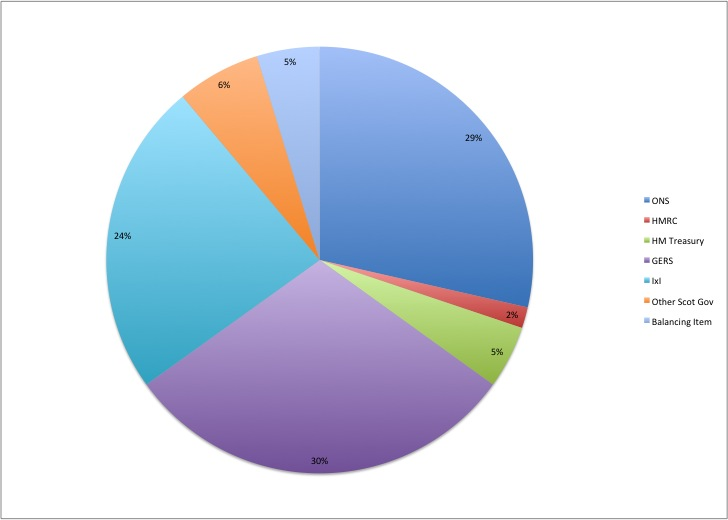
\includegraphics[height=4.3in,width=6in]{incexpsources}
       \else
         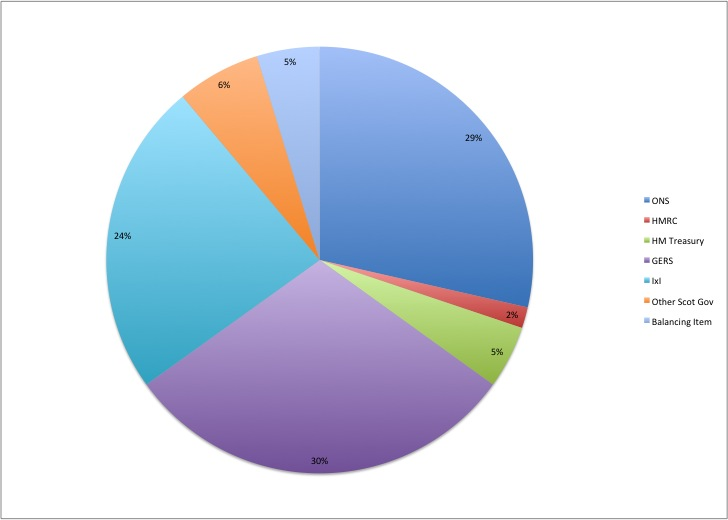
\includegraphics[bb = 92 86 545 742, height=6in]{incexpsources}
       \fi
    \caption{Percentage of data sources in Income and Expenditure Accounts}
    \label{incexpsources}
  \end{center} \label{fig:2.4.1}
\end{figure}


\pagebreak

\pagebreak


%%%%%%%%%%%%%%%%%%%%%%%%%%%%%%%%%%%%%%%%%%%%%%%%%%%%%%%%%%
%SECTION
%%%%%%%%%%%%%%%%%%%%%%%%%%%%%%%%%%%%%%%%%%%%%%%%%%%%%%%%%%
\newpage
\section{Income and Expenditure Accounts - Methodology}
\label{sec:2.5}

\bigskip
\begin{center}
\textbf{\LARGE Households}
\end{center}

\begin{enumerate}


\item \textbf {Income}

\bigskip

The Household income entry is derived from the latest revised figures of Scottish Gross Disposable Household Income (GDHI) for 2009 \cite{ONS2013a}. This data is obtained for Scotland at NUTS2 level covering the variables listed in Table \ref{tab:2.4.1}. The total Household Income figure of \textsterling107,877m is obtained by summing up Operating surplus$/$Mixed income (\textsterling9,437m), Compensation of employees (\textsterling64,645m), Property income received minus paid (\textsterling8,485m - \textsterling551m), Imputed social contributions$/$Social benefits received (\textsterling23,559m), and Other current transfers received minus Other current transfers paid (\textsterling5,102m - \textsterling2,800m).    

\bigskip

\begin{table}[H] \caption{Scottish Gross Disposable Household Income (GDHI) in \textsterling million by component}
\bigskip \begin{scriptsize} \begin{centering} \begin{doublespacing}
% INSERT
    \begin{tabular}{lr}
    \toprule
    Operating surplus$/$Mixed income &          9,437  \bigstrut[t]\\
    Compensation of employees &        64,645  \\
    Property income, received &          8,485  \\
    Primary resources total &        82,566  \bigstrut[b]\\
    Property income, paid &             551  \bigstrut[t]\\
    Primary uses total &             551  \\
    Balance of primary incomes &        82,015  \\
    Imputed social contributions/Social benefits received &        23,559  \bigstrut[b]\\
    Other current transfers, received &          5,102  \bigstrut[t]\\
    Secondary resources total &        28,663  \\
    Current taxes on income, wealth etc. &        13,893  \\
    Social contributions/Social benefits paid &        17,678  \bigstrut[b]\\
    Other current transfers, paid &          2,800  \bigstrut[t]\\
    Secondary uses total &        34,370  \\
    Balance of secondary income & -        5,708  \\
    Gross Disposable Income &        76,307  \bigstrut[b]\\
\bottomrule \end{tabular}%  
\bigskip \begin{flushright} Data sourced from: \cite{ONS2013a}\end{flushright} \label{tab:2.5.1} 
\end{doublespacing} \end{centering} \end{scriptsize} \end{table} \bigskip

\bigskip




\begin{equation}
\begin{split}
\text{Income} =
\text{Total Household Income}_\text{GDHI}
\end{split} \label{eq:2.5.1}
\end{equation}

\begin{equation} \nonumber
110677 = 110677
\end{equation}\\

\item \textbf {Income from Employment}

This is the ``Total intermediate demand'' \text{|| }``Compensation of employees'' from the IO Tables. [Source: Scottish Government (2013a)] \cite{ScottishGovernment2013a}

\begin{equation}
\begin{split}
\text{Income from Employment} =  \\ \\
(\text{Total Intermediate Demand}\|\text{Compensation of Employees})
\end{split} \label{eq:2.5.2}
\end{equation}

\begin{equation} \nonumber
63561 = 63561
\end{equation}\\


\item \textbf {Profit Income (OVA)}

\bigskip

This entry requires that the Gross Operating Surplus for Scotland is identified. Yet, as shown in Table \ref{tab:2.4.1}, data for Scotland is only available as an aggregate comprising of Operating surplus and Mixed income equal in total to \textsterling9,437m. Therefore, this figure has to be disaggregated to identify the Gross Operating Surplus component. This is estimated by using shares derived from 1999 GDHI data which reports these figures individually. There are no alternative datasets available that would allow for a better estimation of Scottish Gross Operating Surplus for 2009. 

\bigskip

Table \ref{tab:2.5.2} illustrates this process. First, the GDHI data for 1999 is obtained \shortcite{Hermannsson2010a}. Next, the the GDHI components are listed. Last, using the Gross Operating Surplus and Gross mixed income shares derived from 1999, the 2009 figures are disaggregated (i.e. \textsterling9437m * (\textsterling3413m / \textsterling3413m + \textsterling2677m) = \textsterling5289m and \textsterling9437 * (\textsterling2677m / \textsterling2677m + \textsterling3413m) = \textsterling4148m). This process yields the required Gross Operating Surplus estimate for Scotland of \textsterling5,289m. Thus, 2009 data (the control total) is disaggregate by using 1999 shares to yield the necessary variables.      

\bigskip

\begin{table}[H] \caption{Scottish Gross Disposable Household Income (GDHI) in \textsterling million by component}
\bigskip \begin{scriptsize} \begin{centering} \begin{doublespacing}
% INSERT
    \begin{tabular}{lrrr}
        \toprule
          & 1999  & 2009  & 2009 using shares \\
        \hline      
    Total household income &              71,296  &               107,877  &               107,877  \\
    Gross operating surplus &                 3,413  &                   9,437  &                   5,289  \\
    Gross mixed income &                 2,677  &   -    &                   4,148  \\
    Compensation of employees &              40,593  &                 64,645  &                 64,645  \\
    Net property income &                 6,591  &                   7,934  &                   7,934  \\
    All pensions &                 8,961  &                 23,559  &                 13,886  \\
    Other social benefits &                 6,242  &   -    &                   9,673  \\
    Net other income &                 2,820  &                   2,302  &                   2,302  \\
    \hline
    Total household disposable income &              48,931  &                 76,307  &                 76,307  \\
\bottomrule \end{tabular}%  
\bigskip \begin{flushright} Data sourced from: \cite{ONS2013a} and \shortcite{Hermannsson2010a}\end{flushright} \label{tab:2.4.2} 
\end{doublespacing} \end{centering} \end{scriptsize} \end{table} \bigskip



\begin{equation}
\begin{split}
\text{Profit Income} = \text{Gross Operating Surplus}_\text{GDHI}
\end{split} \label{eq:2.5.3}
\end{equation}

\begin{equation} \nonumber
5289 = 5289
\end{equation}\\


\item \textbf {Income from Corporations}

This is calculated from three sources. First, taking the Capital Gains Tax receipts as presented in GERS and dividing it by the fixed 18\% Capital Gains Tax Rate for 2008-10 gives an estimate of the actual monetary value of the capital gain received by Scottish households for 2009. 
Second, the total income received by households from corporations is added. This comprises multiplying the share of Scottish GDP, which is calculated using the ratio of total UK GDP at market prices over Scottish GDP at market prices, by the Total of ``UK Private Dividends'' paid out by private non-financial corporations in the UK. In turn this figure is then multiplied by the average (figures are only available for 2008 and 2010) of an individual`s share of total equity on a UK basis, which is used to distinguish the dividend payments received by private shareholders versus, for example, funds. Further, the total income figure is comprised of adding an estimate of the ``Total Private Pensions'' received by Scottish households to the above as well as household`s ``Net Other Income'' from the GDHI. 
Third, the unallocated income from 10 is added in order to balance this part of the Accounts.  \cite{ScotGov2013b,HMRC2013,ONS2011c,ONS2012}


\begin{equation}
\begin{split}
\text{Income from Corporations} =  \\ \\
\text{Total Household Income from Corporations}\\
+\text{Household Income from Capital Gains}\\
+\text{Mixed and Prop Income Unallocated}_\text{IncExp}\\
\end{split} \label{eq:2.5.4}
\end{equation}

\begin{equation} \nonumber
17904 = 15558+1478+869
\end{equation}

\begin{center}
\line(1,0){250}
\end{center}

\textit{where}

\begin{equation} 
\begin{split}
\text{Total Household Income from Corporations} = \\ 
(\text{Scottish GDP Share}*\text{Total UK Private Dividend Payments})\\
*(\text{Individual Share of Total Equity} + \text{Total Private Pension}\\
 + \text{Net Other Income})
\end{split} \label{eq:2.5.5}
\end{equation} 

\begin{equation} \nonumber
15558 = (8.22\% * 85816)*((\frac{10.2\%+11.5\%}{2})+9691+5102)
\end{equation}

\begin{center}
\line(1,0){250}
\end{center}


\begin{equation} 
\begin{split}
\text{Household Income from Capital Gains} = \\ 
(1/4 *\text{Households' Captial Gains Tax Payments}_\text{08-09}\\
+ 3/4 *\text{Households' Captial Gains Tax Payments}_\text{09-10})\\
\div \text{Capital Gains Tax Rate}
\end{split} \label{eq:2.5.6}
\end{equation} 

\begin{equation} \nonumber
1478 = (1/4*572+3/4*164)\div 18\%
\end{equation}

\begin{center}
\line(1,0){250}
\end{center}


\begin{equation} 
\begin{split}
\text{Mixed and Prop Income Unallocated} = \\ 
(\text{Total Household Income}_\text{GDHI}-\text{Total Household Income}_\text{IncExp})\\
\end{split} \label{eq:2.5.7}
\end{equation} 

\begin{equation} \nonumber
869 = 110677-109808
\end{equation}\\

\item \textbf {Income from Government}

The first part of this figure is the annualised ``Social Protection Payments'' to Scottish households and the second one is the ``Public Dividend Payments'' received by Scottish households. The latter is calculated in accordance with the methodology outlined above for ``Private Dividend Payments''. The dividend payments are sourced from non-financial corporations, Central Government and Local Government accounts and are multiplied by the Scottish GDP share as well as the average individual`s share of total equity and further multiplied by the UK Public Dividend payments.  \cite{ScotGov2013b,ONS2011c}

\begin{equation}
\begin{split}
\text{Income from Government} =  \\ \\
(1/4*\text{Total Social Protection}_\text{08-09}\\
+3/4*\text{Total Social Protection}_\text{09-10})\\
+(\text{Scottish GDP Share} \\
*(\text{UK Public Dividends}_\text{Non-Financial Corporations}\\
+\text{UK Public Dividends}_\text{Central Government}\\
+\text{UK Public Dividends}_\text{Local Government})\\
*((\text{Individual's Share of Total Equity}_\text{2008}\\
+\text{Individual's Share of Total Equity}_\text{2009})\div 2))
\end{split} \label{eq:2.5.8}
\end{equation}


\begin{equation} \nonumber
\begin{split}
19835 = (1/4*18653+3/4*20193)\\
+(8.22\%*(25+2214+772)*((10.2\%+11.5\%)\div 2))
\end{split}
\end{equation}\\


\item \textbf {Transfers from RUK}

These transfers are calculated by first, taking the total figure of dividends paid to Scottish households. This figure is calculated by using the share of Scottish Households of total UK Households and multiplying it by ``Total RUK Dividends'' paid to households. The latter figure is based on the average individual`s share of total equity multiplied by the difference between Total UK- and Total Scottish- private dividends in order to obtain the RUK dividend payments to Households in Scotland. 
Second, this is then added to the difference of the ``Compensation of Employees'' according to the GDHI estimates and the actual figure of income from employment as calculated for the Income and Expenditure Account (see 2).
\cite{ONS2011c,ONS2011a,ONS2011b}


\begin{equation}
\begin{split}
\text{Transfers from RUK} =  \\ \\
\text{Total RUK Dividends to Scottish Households}\\
+(\text{Compensation of Employees}_\text{GDHI}\\
-\text{Income from Employment}_\text{IncExp})
\end{split} \label{eq:2.5.9}
\end{equation}

\begin{equation} \nonumber
1852 = 767+(64645-63561)
\end{equation}\\

\begin{center}
\line(1,0){250}
\end{center}

\textit{where}

\begin{equation}
\begin{split}
\text{Total RUK Dividends to Scottish Households}=\\
\text{Scottish Household Share}*\text{Total RUK Dividends to Households}
\end{split} \label{eq:2.5.10}
\end{equation}

\begin{equation}\nonumber
767=8.98\%*8546
\end{equation}


\item \textbf {Transfers from ROW}

The first part of this figure is calculated by multiplying UK employment income from ROW with the OVA for Scotland (see below for breakdown of OVA and OVA repatriated calculations). Added to this is the Scottish share of UK GDP (as shown above) multiplied with the Scottish household share of OVA for UK property and entrepreneurial income and multiplied by the actual amount of the ``UK Property and Entrepreneurial Income''. \cite{ScotGov2013a,ONS2011c,ScotGov2013b}

\begin{equation}
\begin{split}
\text{Transfers from ROW} =  \\ \\
(\text{Scottish Share of UK Total OVA}*\\
\text{UK Employment Income from ROW})\\
+(\text{Scottish Household OVA}*\text{Scottish GDP Share of UK}\\
*\text{UK Property and Entrepreneurial Income})
\end{split} \label{eq:2.5.11}
\end{equation}


\begin{equation} \nonumber
2237 = (143588.31\%)+(169313*15\%*8.22\%)
\end{equation}\\

\item \textbf {Total Household Income}

Totals Figure: Summation of all of the above, excluding the total household income figure obtained from the GDHI (sum: 2 to 7).

\begin{equation}
\begin{split}
\text{Total Household Income} =  \\ \\
(\text{Income from Employment}^\text{Households}_\text{IncExp}\\
+\text{Profit Income (OVA)}^\text{Households}_\text{IncExp}\\
+\text{Income from Corporations}^\text{Households}_\text{IncExp}\\
+\text{Income from Government}^\text{Households}_\text{IncExp}\\
+\text{Transfers from RUK}^\text{Households}_\text{IncExp}\\
+\text{Transfers from ROW}^\text{Households}_\text{IncExp})
\end{split} \label{eq:2.5.12}
\end{equation}

\begin{equation} \nonumber
110677 = 63561+5289+17904+19835+1852+2237
\end{equation}\\


\item \textbf {Mixed and Prop Income Unallocated}

Balancing item equal to the difference of Household Income as presented in the GDHI and the sum of all income figures derived above. This figure gets added into the Income from Corporations as outlined above and is thus zero, due to the two household income figures balancing now. [Source: IncExp Accounts] \cite{ONS2011b}

\begin{equation}
\begin{split}
\text{Income Unallocated} =  \\ \\
\text{Income}^\text{Households}_\text{IncExp}\\
-\text{Income from Employment}^\text{Households}_\text{IncExp}
\end{split} \label{eq:2.5.13}
\end{equation}


\begin{equation} \nonumber
869 = 110677-109808
\end{equation}\\


\pagebreak

\item \textbf {Expenditure}

Totals Figure: Summation of figures presented below, from IO Expenditure to Transfers to ROW (sum: 11 to 16).

\begin{equation}
\begin{split}
\text{Expenditure} =  \\ \\
(\text{IO Expenditure}^\text{Households}_\text{IncExp}\\
+\text{Payments to Corporations}^\text{Households}_\text{IncExp}\\
+\text{Payments to Government}^\text{Households}_\text{IncExp}\\
+\text{Payments to Capital}^\text{Households}_\text{IncExp}\\
+\text{Transfers from RUK}^\text{Households}_\text{IncExp}\\
+\text{Transfers from ROW}^\text{Households}_\text{IncExp})
\end{split} \label{eq:2.5.14}
\end{equation}

\begin{equation} \nonumber
110677 = 74138+9600+21379+5202+238+119
\end{equation}\\


\item \textbf {IO Expenditure}

This cell is made up of ``Households'' and ``Non-Profit Institutions Serving Households'' (NPISHs) – ``Total intermediate consumption at basic prices'' as well as ``Taxes less subsidies on products'' for both sectors. \cite{ScotGov2013a}

\begin{equation}
\begin{split}
\text{IO Expenditure} =  \\ \\
(\text{Final Cons. Expend.}_\text{Households}\|\text{Total Interm. Cons.})\\
+(\text{Final Cons. Expend.}_\text{NPISH}\|\text{Total Interm. Cons.})\\
+(\text{Final Cons. Expend.}_\text{Households}\|\text{Taxes less subsidies on products})\\
+(\text{Final Cons. Expend.}_\text{NPISH}\|\text{Taxes less subsidies on products})
\end{split} \label{eq:2.5.15}
\end{equation}

\begin{equation} \nonumber
74138 = 64890+6568+26803+0
\end{equation}\\


\item \textbf {Payments to Corporations}

Balancing Item: which takes the Total Expenditure and subtracts from it the IO Expenditure, Payments to Government, Payments to Capital, Transfers to RUK and Transfers to ROW (17 – 11,14,15,16).

\begin{equation}
\begin{split}
\text{Payments to Corporations} =  \\ \\
\text{Total Expenditure}^\text{Households}_\text{IncExp}-\text{Transfers to ROW}^\text{Households}_\text{IncExp}\\
-\text{Transfers to RUK}^\text{Households}_\text{IncExp}-\text{Payments to Capital}^\text{Households}_\text{IncExp}\\
-\text{Payments to Government}^\text{Households}_\text{IncExp}-\text{IO Expenditure}^\text{Households}_\text{IncExp}
\end{split} \label{eq:2.5.16}
\end{equation}

\begin{equation} \nonumber
9600 = 110677-119-238-5202-21379-74138
\end{equation}\\


\item \textbf {Payments to Government}

This refers to the annualised tax payments by Scottish households. These taxes are: Income Tax, Capital Gains Tax, Inheritance Tax, Stamp Duties, Half Insurance Premium Tax, Council Tax and Social Security Contributions (NI). \cite{ScotGov2013b}

\begin{equation}
\begin{split}
\text{Payments to Government} =  \\ \\
(1/4*(\text{Income Tax}_\text{08-09}+\text{Capital Gains Tax}_\text{08-09}\\
+(\text{Inheritance Tax}_\text{08-09}+\text{Stamp Duties}_\text{08-09}\\
+(\text{Half Insurance Premium Tax}_\text{08-09}+\text{Council Tax}_\text{08-09}\\
+(\text{Social Security Contributions}_\text{08-09}))\\
+(3/4*(\text{Income Tax}_\text{09-10}+\text{Capital Gains Tax}_\text{09-10}\\
+(\text{Inheritance Tax}_\text{09-10}+\text{Stamp Duties}_\text{09-10}\\
+(\text{Half Insurance Premium Tax}_\text{09-10}+\text{Council Tax}_\text{09-10}\\
+(\text{Social Security Contributions}_\text{09-10}))\\
\end{split} \label{eq:2.5.17}
\end{equation}

\begin{equation} \nonumber
\begin{split}
21379=(1/4*(10642+572+178+594+96+1960+7992))\\
+(3/4*(10364+164+146+516+95+1961+7915))
\end{split}
\end{equation}\\


\item \textbf {Transfers to RUK}

The value of Transfers to ROW (16) is multiplied by two.

\begin{equation}
\begin{split}
\text{Transfers to RUK} =  \\ \\
\text{Transfers to ROW}^\text{Households}_\text{IncExp}*2
\end{split} \label{eq:2.5.18}
\end{equation}

\begin{equation} \nonumber
238 = 119*2
\end{equation}\\


\item \textbf {Transfers to ROW}

This figure is made up of the amount of employee compensation that is paid to the ROW, i.e. the part that is deducted from GDP in order to arrive at GNP figures, times the share of Scottish OVA of Corporate Income (\ref{eq:2.5.84}). \cite{ONS2011c}

\begin{equation}
\begin{split}
\text{Transfers to ROW} =  \\ \\
\text{UK Payments to ROW}*\text{Scottish Corporate Income OVA}
\end{split} \label{eq:2.5.19}
\end{equation}

\begin{equation} \nonumber
119 = 1435*8.31\%
\end{equation}\\


\item \textbf {Payments to Capital (Savings)}

The Total Expenditure (18) is multiplied by the Household Saving rate as given by SNAP, in order to obtain an estimate for this cell. \cite{ScotGov2013c}

\begin{equation}
\begin{split}
\text{Payments to Capital} =  \\ \\
\text{Total Household Income}^\text{Households}_\text{IncExp}\\
+\text{Household Savings Rate}_\text{SNAP}
\end{split} \label{eq:2.5.20}
\end{equation}

\begin{equation} \nonumber
5202 = 110677*0.047
\end{equation}\\


\item \textbf {Total Expenditure}

Corresponding Figure: Equal to the Total Household Income (9).

\begin{equation}
\begin{split}
\text{Total Expenditure} =  \\ \\
\text{Total Household Income}^\text{Households}_\text{IncExp}
\end{split} \label{eq:2.5.21}
\end{equation}

\begin{equation} \nonumber
110677 = 110677
\end{equation}\\



\pagebreak

\begin{center}
\textbf{\LARGE Corporations}
\end{center}

\item \textbf {Income}

Totals Figure: Equal to all of the items below in this section (19 to 23).

\begin{equation}
\begin{split}
\text{Income} =  \\ \\
\text{Profit Income}^\text{Corporations}_\text{IncExp}\\
+\text{Income from Households}^\text{Corporations}_\text{IncExp}\\
+\text{Income from Government}^\text{Corporations}_\text{IncExp}\\
+\text{Income from RUK}^\text{Corporations}_\text{IncExp}\\
+\text{Income from ROW}^\text{Corporations}_\text{IncExp}
\end{split} \label{eq:2.5.22}
\end{equation}

\begin{equation} \nonumber
56175 = 29456+9600+5191+5964+5964
\end{equation}\\

\item \textbf {Profit Income (OVA)}

Taking the ``Total Intermediate Demand'' – ``Gross Operating Surplus'', the OVA of both Households and Government (3 and 31) are deducted from it from it.  \cite{ScotGov2013a,ONS2011b}

\begin{equation}
\begin{split}
\text{Profit Income} =  \\ \\
\text{Total Intermediate Demand}\|\text{Gross Operating Surplus}\\
-\text{Profit Income}^\text{Households}_\text{IncExp}-\text{Profit Income}^\text{Government}_\text{IncExp}
\end{split} \label{eq:2.5.23}
\end{equation}

\begin{equation} \nonumber
29456 = 38441-5289-3697
\end{equation}\\


\item \textbf {Income from Households}

Corresponding Figure: Equal to Payments to Corporations under Household Expenditure (12).

\begin{equation}
\begin{split}
\text{Income from Households} =  \\ \\
\text{Payments to Corporations}^\text{Households}_\text{IncExp}
\end{split} \label{eq:2.5.24}
\end{equation}

\begin{equation} \nonumber
9600 = 9600
\end{equation}\\


\item \textbf {Income from Government}

Corresponding Figure: Equal to Payments to Corporations under Government Expenditure (39).

\begin{equation}
\begin{split}
\text{Income from Government} =  \\ \\
\text{Payments to Corporations}^\text{Government}_\text{IncExp}
\end{split} \label{eq:2.5.25}
\end{equation}

\begin{equation} \nonumber
5191 = 5191
\end{equation}\\


\item \textbf {Income from RUK}

Using the Scottish share of UK property and entrepreneurial income (see \ref{eq:2.5.82}), it is multiplied by the corporate share of OVA. One half of this figure is used for this cell and the other for the one below (23). \cite{ONS2011c}

\begin{equation}
\begin{split}
\text{Income from RUK} =  \\ \\
1/2*\text{Corporate OVA Share}\\
*\text{Scottish Share of UK Property and Entrepreneurial Income}
\end{split} \label{eq:2.5.26}
\end{equation}

\begin{equation} \nonumber
5964 = 84.8\%*14070*1/2
\end{equation}\\


\item \textbf {Income from ROW}

Other half of figure calculated in first part of 22.

\begin{equation}
\begin{split}
\text{Income from RUK} =  \\ \\
1/2*\text{Corporate OVA Share}\\
*\text{Scottish Share of UK Property and Entrepreneurial Income}
\end{split} \label{eq:2.5.27}
\end{equation}

\begin{equation} \nonumber
5964 = 84.8\%*14070*1/2
\end{equation}\\


\pagebreak

\item \textbf {Expenditure}

Totals Figure: cells below (25 to 29).

\begin{equation}
\begin{split}
\text{Expenditure} =  \\ \\
\text{Payments to Households}^\text{Corporations}_\text{IncExp}\\
+\text{Payments to Government}^\text{Corporations}_\text{IncExp}\\
+\text{Transfers to RUK}^\text{Corporations}_\text{IncExp}\\
+\text{Transfers to ROW}^\text{Corporations}_\text{IncExp}\\
+\text{Payments to Capital}^\text{Corporations}_\text{IncExp}
\end{split} \label{eq:2.5.28}
\end{equation}

\begin{equation} \nonumber
56175 = 17904+5248+3768+4560+24695
\end{equation}\\


\item \textbf {Payments to Households}

Corresponding Figure: Equal to Household Income from Corporations (4).

\begin{equation}
\begin{split}
\text{Payments to Households} =  \\ \\
\text{Income from Corporations}^\text{Households}_\text{IncExp}
\end{split} \label{eq:2.5.29}
\end{equation}

\begin{equation} \nonumber
17904 = 17904
\end{equation}\\


\item \textbf {Payments to Government}

These are the annualised corporate taxes: Corporation Tax, (Windfall Tax) Half Insurance Premium Tax, Landfill Tax, Non-Domestic Rates, Other Taxes and Royalties, Interest and Dividends \cite{ScotGov2013b}

\begin{equation}
\begin{split}
\text{Payments to Government} =  \\ \\
(1/4*(\text{Corporation Tax}_\text{08-09}+\text{Half Insurance Premium Tax}_\text{08-09}\\
+(\text{Landfill Tax}_\text{08-09}+\text{Non-Domestic Rates}_\text{08-09}\\
+(\text{Other Taxes and Royalties}_\text{08-09}+\text{Interest and Dividends}_\text{08-09}\\
+(3/4*(\text{Corporation Tax}_\text{09-10}+\text{Half Insurance Premium Tax}_\text{09-10}\\
+(\text{Landfill Tax}_\text{09-10}+\text{Non-Domestic Rates}_\text{09-10}\\
+(\text{Other Taxes and Royalties}_\text{09-10}+\text{Interest and Dividends}_\text{09-10}\\
\end{split} \label{eq:2.5.30}
\end{equation}

\begin{equation} \nonumber
\begin{split}
5248 = (1/4*(2841+96+82+1736+250+608))\\
+(3/4(2680+95+85+1822+212+233))
\end{split}
\end{equation}\\


\item \textbf {Transfers to RUK}

Equal to OVA repatriated to RUK (see \ref{eq:2.5.80}). \cite{ScotGov2012}\\

\begin{equation}
\begin{split}
\text{Transfers to RUK} =  \\ \\
\text{Share of OVA Repatriated to RUK}*\text{Profit Income}^\text{Corporations}_\text{IncExp}
\end{split} \label{eq:2.5.31}
\end{equation}

\begin{equation} \nonumber
3768 = 13\%829456
\end{equation}\\


\item \textbf {Transfers to ROW}

Equal to OVA repatriated to ROW (see \ref{eq:2.5.81}). \cite{ScotGov2012}

\begin{equation}
\begin{split}
\text{Transfers to ROW} =  \\ \\
\text{Share of OVA Repatriated to ROW}*\text{Profit Income}^\text{Corporations}_\text{IncExp}
\end{split} \label{eq:2.5.32}
\end{equation}

\begin{equation} \nonumber
4560 = 15\%*829456
\end{equation}\\


\item \textbf {Payments to Capital (Savings)}

Balancing Item: This figure is derived by summing up the ``Gross Fixed Capital Formation'' (GFCF) for all Public Sectors in the IO Tables and then deducting the sum of the ``Taxes less subsidies on production'' for these sectors. The Public Sectors are: Water and Sewerage, Public Administration and Defence, Education, Health, Residential Care and Social Work. \cite{ScotGov2013a}

\begin{equation}
\begin{split}
\text{Payments to Capital} =  \\ \\
\text{Income}^\text{Corporations}_\text{IncExp}\\
-\text{Payments to Households}^\text{Corporations}_\text{IncExp}\\
-\text{Payments to Government}^\text{Corporations}_\text{IncExp}\\
-\text{Transfers to RUK}^\text{Corporations}_\text{IncExp}\\
-\text{Transfers to ROW}^\text{Corporations}_\text{IncExp}
\end{split} \label{eq:2.5.33}
\end{equation}

\begin{equation} \nonumber
24695 = 56175-17904-5248-3768-4560
\end{equation}\\


\pagebreak

\begin{center}
\textbf{\LARGE Government}
\end{center}

\item \textbf {Income}

Totals Figure: Sum of cells below (31 to 35).

\begin{equation}
\begin{split}
\text{Income} =  \\ \\
\text{Profit Income}^\text{Government}_\text{IncExp}\\
+\text{Net Commodity Tax}^\text{Government}_\text{IncExp}\\
+\text{Income from Households}^\text{Government}_\text{IncExp}\\
+\text{Income from Corporations}^\text{Government}_\text{IncExp}
\end{split} \label{eq:2.5.34}
\end{equation}

\begin{equation} \nonumber
63530 = 3697+13165+21379+5248+10041
\end{equation}\\


\item \textbf {Profit Income (OVA)}

Equal to ``Taxes less subsidies on production'' for all public sectors (see 30).  \cite{ScotGov2013a}

\begin{equation}
\begin{split}
\text{Profit Income} =  \\ \\
\text{Water and Sewerage}\|\text{Gross Operating Surplus}\\
+\text{Public Administration and Defence}\|\text{Gross Operating Surplus}\\
+\text{Education}\|\text{Gross Operating Surplus}\\
+\text{Health}\|\text{Gross Operating Surplus}\\
+\text{Residential Care}\|\text{Gross Operating Surplus}\\
+\text{Social Work}\|\text{Gross Operating Surplus}
\end{split} \label{eq:2.5.35}
\end{equation}

\begin{equation} \nonumber
3697 = 710+865+463+817+590+253
\end{equation}\\


\item \textbf {Net Commodity Taxes}

This cell is the sum of ``Total Intermediate Deman''” – ``Taxes less subsidies on production'' and ``Total Demand for Products'' – ``Taxes less subsidies on products''. \cite{ScotGov2013a}\\

\begin{equation}
\begin{split}
\text{Net Commodity Taxes} =  \\ \\
\text{Total Intermediate Demand}\|\text{Taxes less Subsidies on Production}\\
+\text{Total Demand for Products}\|\text{Taxes less Subsidies on Products}\\
\end{split} \label{eq:2.5.36}
\end{equation}

\begin{equation} \nonumber
13165 = 1232+11933
\end{equation}\\


\item \textbf {Income from Households}

Corresponding Figure: Equal to Payments to Government under Household Expenditure (13).

\begin{equation}
\begin{split}
\text{Income from Households} =  \\ \\
\text{Payments to Government}^\text{Households}_\text{IncExp}
\end{split} \label{eq:2.5.37}
\end{equation}

\begin{equation} \nonumber
21379 = 21379
\end{equation}\\


\item \textbf {Income from Corporations}

Corresponding Figure: Equal to Payments to Government under Corporations Expenditure (26).

\begin{equation}
\begin{split}
\text{Income from Coporations} =  \\ \\
\text{Payments to Government}^\text{Corporations}_\text{IncExp}
\end{split} \label{eq:2.5.38}
\end{equation}

\begin{equation} \nonumber
5248 = 5248
\end{equation}\\


\item \textbf {Income from RUK}

Balancing Item: Total Gov. Income Balancing Total (36) minus the sum of Profit Income, Net Commodity Taxes, Income from Households and Income from Corporations (31 to 34).\\

\begin{equation}
\begin{split}
\text{Income from RUK} =  \\ \\
\text{Total Government Income Balancing}\\
-\text{Profit Income}^\text{Government}_\text{IncExp}\\
-\text{Net Commodity Taxes}^\text{Government}_\text{IncExp}\\
-\text{Income from Households}^\text{Government}_\text{IncExp}\\
-\text{Income from Corporations}^\text{Government}_\text{IncExp}
\end{split} \label{eq:2.5.39}
\end{equation}

\begin{equation} \nonumber
20041 = 63530-3697-13165-21379-5248
\end{equation}\\


\item \textbf {Total Government Income Balancing Total}

Corresponding Figure: Equal to Total Government Expenditure Balancing Total (43).\\

\begin{equation}
\begin{split}
\text{Total Government Income} =  \\ \\
\text{Total Government Expenditure Balancing Total}^\text{Government}_\text{IncExp}
\end{split} \label{eq:2.5.40}
\end{equation}

\begin{equation} \nonumber
63530 = 63530
\end{equation}\\



\pagebreak

\item \textbf {Expenditure}

Totals Figure: Summation for cells below (38 to 42).\\

\begin{equation}
\begin{split}
\text{Expenditure} =  \\ \\
\text{IO Expenditure}^\text{Government}_\text{IncExp}\\
+\text{Payments to Corporations}^\text{Government}_\text{IncExp}\\
+\text{Payments to Households}^\text{Government}_\text{IncExp}\\
+\text{Transfers to RUK}^\text{Government}_\text{IncExp}\\
+\text{Payments to Capital}^\text{Government}_\text{IncExp}
\end{split} \label{eq:2.5.41}
\end{equation}

\begin{equation} \nonumber
63530 = 30017+5191+19835+8368+119
\end{equation}\\


\item \textbf {IO Expenditure}

This is the ``Central Government'' and ``Local Governments'' – ``Total intermediate consumption at basic prices''. \cite{ScotGov2013a}

\begin{equation}
\begin{split}
\text{IO Expenditure} =  \\ \\
\text{Central Government}\|\text{Total Intermediate Consumption at basic Prices}\\
+\text{Local Government}\|\text{Total Intermediate Consumption at basic Prices}
\end{split} \label{eq:2.5.42}
\end{equation}

\begin{equation} \nonumber
30017 = 19462+10555
\end{equation}\\


\item \textbf {Payments to  Corporations}

Balancing Item:  Total Government Expenditure Balancing Total (44) minus IO Expenditure, Payments to Households, Transfers to RUK and Payments to Capital (Savings) (38, 40, 41, 42).

\begin{equation}
\begin{split}
\text{Payments to Corporations} =  \\ \\
\text{Total Government Expenditure Balancing Total}^\text{Government}_\text{IncExp}\\
-\text{IO Expenditure}^\text{Government}_\text{IncExp}\\
+\text{Payments to Households}^\text{Government}_\text{IncExp}\\
+\text{Transfers to RUK}^\text{Government}_\text{IncExp}\\
+\text{Payments to Capital}^\text{Government}_\text{IncExp}
\end{split} \label{eq:2.5.43}
\end{equation}

\begin{equation} \nonumber
5191 = 63530-30017-19835-8368-119
\end{equation}\\


\item \textbf {Payments to Households}

Corresponding Figure: Income from Government from the Household Income Accounts (5).\\

\begin{equation}
\begin{split}
\text{Payments to Households} =  \\ \\
\text{Income from Government}^\text{Households}_\text{IncExp}
\end{split} \label{eq:2.5.44}
\end{equation}

\begin{equation} \nonumber
19835 = 19835
\end{equation}\\


\item \textbf {Transfers to RUK}

This is the annualised estimated non-identifiable Government Expenditure, which is based on the Scottish population share of the UK Total non-identifiable public spending. \cite{ScotGov2013b}

\begin{equation}
\begin{split}
\text{Transfers to RUK} =  \\ \\
1/4*\text{Estimated Non-Identifiable Expenditure}_\text{08-09}\\
+3/4\text{Estimated Non-Identifiable Expenditure}_\text{09-10}
\end{split} \label{eq:2.5.45}
\end{equation}

\begin{equation} \nonumber
8368 = 1/4*8174+3/4*8432
\end{equation}\\


\item \textbf {Payments to Capital (Savings)}

This is the sum of ``Gross Fixes Capital Formation'' for all Public Sectors, which is then subtracted by ``Taxes less subsidies on production'' for these sectors. \cite{ScotGov2013a}\\

\begin{equation}
\begin{split}
\text{Payments to Capital} =  \\ \\
(\text{Gross Fixed Capital Formation}\|\text{Water and Sewerage}\\
+\text{Gross Fixed Capital Formation}\|\text{Public Administration and Defence}\\
+\text{Gross Fixed Capital Formation}\|\text{Education}\\
+\text{Gross Fixed Capital Formation}\|\text{Health}\\
+\text{Gross Fixed Capital Formation}\|\text{Residential Care}\\
+\text{Gross Fixed Capital Formation}\|\text{Social Work})\\
-(\text{Water and Sewerage}\|\text{Taxes less Subsidies on Production}\\
+\text{Public Administration and Defence}\|\text{Taxes less Subsidies on Production}\\
+\text{Education}\|\text{Taxes less Subsidies on Production}\\
+\text{Health}\|\text{Taxes less Subsidies on Production}\\
+\text{Residential Care}\|\text{Taxes less Subsidies on Production}\\
+\text{Social Work}\|\text{Taxes less Subsidies on Production})
\end{split} \label{eq:2.5.46}
\end{equation}

\begin{equation} \nonumber
\begin{split}
119 = (1+174+7+0+0+1)\\
-(28+0+18+11+3+4)
\end{split}
\end{equation}\\


\item \textbf {Total Government Expenditure Balancing Total}

This is the annualised ``Total Identifiable Expenditure'' of the Scottish Government plus the non-identifiable estimate (see 41). Then, the annualised ``Total managed expenditure'', ``Total Identifiable''- and ``Total non-identifiable Expenditure'' of the UK is multiplied by the Scottish population share of the UK Total population and then taken off the two former sums of Public Sector spending in Scotland. \cite{HMTR2012,ONS2011a}\\

\begin{equation}
\begin{split}
\text{Total Government Expenditure} =  \\ \\
(1/4 * \text{Total Identifiable Expenditure}_{08-09} \\
+ 3/4 * \text{Total Identifiable Expenditure}_{09-10})\\
+ (1/4 * \text{Total Non-Identifiable Expenditure}_{08-09} \\
+ 3/4 * \text{Total Non-Identifiable Expenditure}_{09-10}) \\
( 1/4 * \text{Scot. Pop. Share} * ( \text{Total Man. Exp.}^{UK}_{08-09} \\
- \text{Total Ident. Exp.}^{UK}_{08-09} \\
- \text{Total Man. Non-Ident.}^{UK}_{08-09})) \\
( 1/4 * \text{Scot. Pop. Share} * ( \text{Total Man. Exp.}^{UK}_{09-10} \\
- \text{Total Ident. Exp.}^{UK}_{09-10} \\
- \text{Total Man. Non-Ident.}^{UK}_{09-10}))
\end{split} \label{eq:2.5.47}
\end{equation}


\begin{equation} \nonumber
\begin{split}
63530 = (1/4*(50779+8174))+(3/4*(53617+8432))\\
+(1/4*8.41\%*(629745-515734-87697))\\
+(3/4*8.41\%*(670150-559134-84021))
\end{split}
\end{equation}\\


\pagebreak


\begin{center}
\textbf{\LARGE Capital}
\end{center}

\item \textbf {Income}

Totals Figure: Sum of cells below (45 to 48).

\begin{equation}
\begin{split}
\text{Income} =  \\ \\
\text{Households}^\text{Capital}_\text{IncExp}\\
+\text{Corporations}^\text{Capital}_\text{IncExp}\\
+\text{Government}^\text{Capital}_\text{IncExp}\\
+\text{RUK/ROW}^\text{Capital}_\text{IncExp}
\end{split} \label{eq:2.5.48}
\end{equation}

\begin{equation} \nonumber
19930 = 5202+24695+119+(-10086)
\end{equation}\\


\item \textbf {Households)}

Corresponding Figure: Payments to Capital of the Household Expenditure Account (14).

\begin{equation}
\begin{split}
\text{Households} =  \\ \\
\text{Payments to Capital}^\text{Households}_\text{IncExp}
\end{split} \label{eq:2.5.49}
\end{equation}

\begin{equation} \nonumber
5202 = 5202
\end{equation}\\


\item \textbf {Corporate}

Corresponding Figure: Payments to Capital (savings) of the Corporation Expenditure Account (29).

\begin{equation}
\begin{split}
\text{Corporate} =  \\ \\
\text{Payments to Capital}^\text{Corporations}_\text{IncExp}
\end{split} \label{eq:2.5.50}
\end{equation}

\begin{equation} \nonumber
24695 = 24695
\end{equation}\\


\item \textbf {Government}

Corresponding Figure: Payments to Capital (savings) of the Government Expenditure Account (42).

\begin{equation}
\begin{split}
\text{Government} =  \\ \\
\text{Payments to Capital}^\text{Government}_\text{IncExp}
\end{split} \label{eq:2.5.51}
\end{equation}

\begin{equation} \nonumber
119 = 119
\end{equation}\\


\item \textbf {RUK/ROW}

Corresponding Figure: Surplus/Deficit of the External Expenditure Account (66).

\begin{equation}
\begin{split}
\text{RUK/ROW} =  \\ \\
\text{Total Income}^\text{External}_\text{IncExp}\\
-\text{Total Expenditure}^\text{External}_\text{IncExp}
\end{split} \label{eq:2.5.52}
\end{equation}

\begin{equation} \nonumber
-10086 = 90808-100894
\end{equation}\\


\pagebreak

\item \textbf {Expenditure}

Corresponding Figure: IO Expenditure (50).
    
\begin{equation}
\begin{split}
\text{Expenditure} =  \\ \\
\text{IO Expenditure}^\text{Capital}_\text{IncExp}
\end{split} \label{eq:2.5.53}
\end{equation}

\begin{equation} \nonumber
19930 = 19930
\end{equation}\\


\item \textbf {IO Expenditure}

This is the sum of ``Total Gross Capital Formation'' – ``Total intermediate consumption at basic prices'' and ``Total Gross Capital Formation'' – ``Taxes less subsidies on products''. \cite{ScotGov2013a}

\begin{equation}
\begin{split}
\text{IO Expenditure} =  \\ \\
\text{Total Gross Capital Formation}\|\text{Total Interm. Consumption at Basic Prices}\\
+\text{Total Gross Capital Formation}\|\text{Taxes Less Subsidies on Products}
\end{split} \label{eq:2.5.54}
\end{equation}

\begin{equation} \nonumber
19930 = 18453+1495
\end{equation}\\



\pagebreak


\begin{center}
\textbf{\LARGE External}
\end{center}

\item \textbf {UK Income from Scotland}

Totals Figure: This is the sum of the two cells below: Goods \& Services and Transfers (52 \& 53).\\

\begin{equation}
\begin{split}
\text{UK Income from Scotland} =  \\ \\
\text{Goods \& Services}^\text{External}_\text{IncExp}\\
+\text{Transfers}^\text{External}_\text{IncExp}
\end{split} \label{eq:2.5.55}
\end{equation}

\begin{equation} \nonumber
67133 = 54759+12374
\end{equation}\\


\item \textbf {Goods \& Services}

This is the “Total Demand for Products” from RUK. \cite{ScotGov2013a}

\begin{equation}
\begin{split}
\text{Goods \& Services} =  \\ \\
\text{Total Demand for Products}\|\text{Imports from Rest of UK}
\end{split} \label{eq:2.5.56}
\end{equation}

\begin{equation} \nonumber
54759 = 54759
\end{equation}\\


\item \textbf {Transfers}

This is the sum of: ``Transfers to RUK'' from the Household Expenditure Account, ``Transfers to RUK'' from the Corporations Expenditure Account and the ``Transfers to RUK'' from the Government Expenditure Account (6, 22, 35).\\

\begin{equation}
\begin{split}
\text{Transfers} =  \\ \\
\text{UK Income from Scotland} =  \\ \\
\text{Transfers to RUK}^\text{Households}_\text{IncExp}\\
+\text{Transfers to RUK}^\text{Corporations}_\text{IncExp}\\
+\text{Transfers to RUK}^\text{Government}_\text{IncExp}
\end{split} \label{eq:2.5.57}
\end{equation}

\begin{equation} \nonumber
12374 = 238+3768+8368
\end{equation}\\


\item \textbf {ROW Income from Scotland}

Totals Figure: This is the sum of the two cells below: Goods \& Services and Transfers (55 \& 56).\\

\begin{equation}
\begin{split}
\text{ROW Income from Scotland} =  \\ \\
\text{Goods \& Services}^\text{External}_\text{IncExp}\\
+\text{Transfers}^\text{External}_\text{IncExp}
\end{split} \label{eq:2.5.58}
\end{equation}

\begin{equation} \nonumber
23676 = 18997+4697
\end{equation}\\


\item \textbf {Goods \& Services}

This is the ``Total Demand for Products'' – ``ROW''. \cite{ScotGov2013a}

\begin{equation}
\begin{split}
\text{Goods \& Services} =  \\ \\
\text{Total Demand for Products}\|\text{Imports from ROW}
\end{split} \label{eq:2.5.59}
\end{equation}

\begin{equation} \nonumber
18997 = 18997
\end{equation}\\


\item \textbf {Transfers}

This is the sum of: ``Transfers to ROW'' from the Household Expenditure Account and ``Transfers to ROW'' from the Corporations Expenditure Account (7 \& 23).\\

\begin{equation}
\begin{split}
\text{Transfers} =  \\ \\
\text{Transfers to ROW}^\text{Households}_\text{IncExp}\\
+\text{Transfers to RUK}^\text{Corporations}_\text{IncExp}
\end{split} \label{eq:2.5.60}
\end{equation}

\begin{equation} \nonumber
4679 = 119+4560
\end{equation}\\


\item \textbf {Total Income}

Totals Figure: This is the sum of the two cells above: ``UK income from Scotland'' and ``ROW income from Scotland'' (51 \& 54).\\

\begin{equation}
\begin{split}
\text{Total Income} =  \\ \\
\text{UK Income from Scotland}^\text{External}_\text{IncExp}\\
+\text{ROW Income from Scotland}^\text{External}_\text{IncExp}
\end{split} \label{eq:2.5.61}
\end{equation}

\begin{equation} \nonumber
90808 = 67133+23676
\end{equation}\\



\pagebreak

\item \textbf {UK Expenditure in Scotland}

Totals Figure: This is the sum of the two cells below: Goods \& Services and Transfers (59 \& 60).\\

\begin{equation}
\begin{split}
\text{UK Expenditure in Scotland} =  \\ \\
\text{Goods \& Services}^\text{External}_\text{IncExp}\\
+\text{Transfers}^\text{External}_\text{IncExp}
\end{split} \label{eq:2.5.62}
\end{equation}

\begin{equation} \nonumber
70595 = 42739+27857
\end{equation}\\


\item \textbf {Goods \& Services}

This is the ``Total intermediate consumption at basic prices'' – ``Rest of UK exports''. \cite{ScotGov2013a}\\

\begin{equation}
\begin{split}
\text{Goods \& Services} =  \\ \\
\text{Rest of UK Exports}\|\text{Total Interm. Consumption at Basic Prices}
\end{split} \label{eq:2.5.63}
\end{equation}

\begin{equation} \nonumber
42759 = 42759
\end{equation}\\


\item \textbf {Transfers}

This is the sum of: ``Transfers from RUK'' from the Household Income Account, ``Income from RUK'' from the Corporations Income Account and ``Income from RUK'' from the Government Income Account (15, 27, 41).

\begin{equation}
\begin{split}
\text{Transfers} =  \\ \\
\text{Transfers from RUK}^\text{Households}_\text{IncExp}\\
+\text{Income from RUK}^\text{Corporations}_\text{IncExp}\\
+\text{Income from RUK}^\text{Government}_\text{IncExp}
\end{split} \label{eq:2.5.64}
\end{equation}

\begin{equation} \nonumber
27857 = 1852+5964+20041
\end{equation}\\


\item \textbf {ROW Expenditure in Scotland}

Totals Figure: This is the sum of the two cells below: Goods \& Services and Transfers.

\begin{equation}
\begin{split}
\text{ROW Expenditure in Scotland} =  \\ \\
\text{Goods \& Services}^\text{External}_\text{IncExp}\\
+\text{Transfers}^\text{External}_\text{IncExp}
\end{split} \label{eq:2.5.65}
\end{equation}

\begin{equation} \nonumber
27378 = 19178+8201
\end{equation}\\


\item \textbf {Goods \& Services}

This is the ``Total intermediate consumption at basic prices'' – ``Rest of world exports''. \cite{ScotGov2013a}

\begin{equation}
\begin{split}
\text{Goods \& Services} =  \\ \\
\text{Rest of World Exports}\|\text{Total Interm. Consumption at Basic Prices}
\end{split} \label{eq:2.5.66}
\end{equation}

\begin{equation} \nonumber
19178 = 19178
\end{equation}\\


\item \textbf {Transfers}

This is the sum of: ``Transfers from ROW'' from the Household Income Account and ``Income from ROW'' from the Corporations Income Account (16 \& 28).

\begin{equation}
\begin{split}
\text{Transfers} =  \\ \\
\text{Transfers from ROW}+\text{Income from ROW}
\end{split} \label{eq:2.5.67}
\end{equation}

\begin{equation} \nonumber
8201 = 2237+5964
\end{equation}\\



\item \textbf {Tourist Expenditure in Scotland}

This is the sum of the ``Non-resident household expenditure in Scotland'' (under ``Final consumption expenditure'') - ``Total intermediate consumption at basic prices'' and ``Taxes less subsidies on products''. \cite{ScotGov2013a}

\begin{equation}
\begin{split}
\text{Tourist Expenditure in Scotland} =  \\ \\
\text{Final Consumption Expenditure Non-Resident}\\
\text{Household Expenditure in Scotland}\\
\|\text{Total Interm. Consumption at Basic Prices}\\
\text{Final Consumption Expenditure Non-Resident}\\
\text{Household Expenditure in Scotland}\\
\|\text{Taxes Less Subsidies on Products}
\end{split} \label{eq:2.5.68}
\end{equation}

\begin{equation} \nonumber
2921 = 2599+322
\end{equation}\\


\item \textbf {Total Expenditure}

This is the sum of the above cells: ``UK expenditure in Scotland'', ``ROW expenditure in Scotland'' and ``Tourist expenditure in Scotland''.

\begin{equation}
\begin{split}
\text{Total Expenditure} =  \\ \\
\text{UK Expenditure in Scotland}^\text{External}_\text{IncExp}\\
+\text{ROW Expenditure in Scotland}^\text{External}_\text{IncExp}\\
+\text{Tourist Expenditure in Scotland}^\text{External}_\text{IncExp}
\end{split} \label{eq:2.5.69}
\end{equation}

\begin{equation} \nonumber
100894 = 70595+27378+2921
\end{equation}\\


\item \textbf {Surplus/Deficit}

This is the balance of the External Accounts’ ``Total income'' minus ``Total expenditure'' (57 - 65).

\begin{equation}
\begin{split}
\text{Surplus/Deficit} =  \\ \\
\text{Total Income}^\text{External}_\text{IncExp}\\
-\text{Total Expenditure}^\text{External}_\text{IncExp}
\end{split} \label{eq:2.5.70}
\end{equation}

\begin{equation} \nonumber
-10086 = 90808-100894
\end{equation}\\



\pagebreak


\begin{center}
\textbf{\LARGE Goods and Services Trade Balance}
\end{center}

\item \textbf {RUK}

This is the balance of the ``Goods and Services'' of ``UK expenditure in Scotland'' minus those of ``UK income from Scotland'' (59 - 51).

\begin{equation}
\begin{split}
\text{Goods \& Services Trade Balance with RUK} =  \\ \\ 
\text{RUK Goods \& Services Expenditure in Scotland}^\text{External}_\text{IncExp}\\
-\text{RUK Goods \& Services Income from Scotland}^\text{External}_\text{IncExp}
\end{split} \label{eq:2.5.71}
\end{equation}

\begin{equation} \nonumber
-12020 = 42739-54759
\end{equation}\\


\item \textbf {ROW}

This is the balance of the ``Goods and Services'' of ``ROW expenditure in Scotland'' minus those of ``ROW income from Scotland'' (62 - 55).

\begin{equation}
\begin{split}
\text{Goods \& Services Trade Balance with ROW} =  \\ \\ 
\text{ROW Goods \& Services Expenditure in Scotland}^\text{External}_\text{IncExp}\\
-\text{ROW Goods \& Services Income from Scotland}^\text{External}_\text{IncExp}
\end{split} \label{eq:2.5.72}
\end{equation}

\begin{equation} \nonumber
181 = 19178-18997
\end{equation}\\



\pagebreak

\item \textbf {RUK}

Taking the ``UK expenditure in Scotland'' from the External Accounts, the ``Tourist expenditure in Scotland'' is added to it. This is then multiplied by the share attributed to UK versus ROW tourist and subsequently subtracted by ``UK income from Scotland'' (58,64,51).  \cite{ONS2010a}\\

\begin{equation}
\begin{split}
\text{Total Balance of Payments RUK} =  \\ \\
\text{RUK Expenditure in Scotland}^\text{External}_\text{IncExp}\\
+(\text{RUK Share of Tourist Expenditure in Scotland}\\
*\text{Tourist  Expenditure in Scotland}^\text{External}_\text{IncExp})\\
-\text{RUK Income from Scotland}^\text{External}_\text{IncExp}
\end{split} \label{eq:2.5.73}
\end{equation}

\begin{equation} \nonumber
5215 = 70595+(0.6*2921)-67133
\end{equation}\\


\item \textbf {ROW}

Taking the ``ROW expenditure in Scotland'' from the External Accounts, the ``Tourist expenditure in Scotland'' is added to it. This is then multiplied by the share attributed to ROW versus UK tourist and subsequently subtracted by ``ROW income from Scotland'' (61,64,54). \cite{ONS2010a}

\begin{equation}
\begin{split}
\text{Total Balance of Payments ROW} =  \\ \\
\text{ROW Expenditure in Scotland}^\text{External}_\text{IncExp}\\
+(\text{ROW Share of Tourist Expenditure in Scotland}\\
*\text{Tourist  Expenditure in Scotland}^\text{External}_\text{IncExp})\\
-\text{ROW Income from Scotland}^\text{External}_\text{IncExp}
\end{split} \label{eq:2.5.74}
\end{equation}

\begin{equation} \nonumber
4871 = 27378+(0.4*2921)-23676
\end{equation}\\


\item \textbf {Total BOP}

Totals Figure: This is the sum of the two cells above (69 \& 70).

\begin{equation}
\begin{split}
\text{Total Balance of Payments} =  \\ \\
\text{RUK Total Balance of Payments}+\text{ROW Total Balance of Payments}
\end{split} \label{eq:2.5.75}
\end{equation}

\begin{equation} \nonumber
10086 = 5215+4871
\end{equation}\\



\pagebreak

\begin{center}
\textbf{\LARGE External Balance}
\end{center}

\item \textbf {RUK Total Flows Balance}

This is the balance of ``UK income from Scotland'' minus ``UK expenditure in Scotland'' (51 - 58).

\begin{equation}
\begin{split}
\text{RUK Total Flows Balance} =  \\ \\
\text{RUK Income from Scotland}- \text{RUK Expenditure in Scotland}
\end{split} \label{eq:2.5.76}
\end{equation}

\begin{equation} \nonumber
-3462 = 67133-70595
\end{equation}\\


\item \textbf {ROW Total Flows Balance}

This is the balance of ``ROW income from Scotland'' minus ``ROW expenditure in Scotland'' (54 - 61).

\begin{equation}
\begin{split}
\text{ROW Total Flows Balance} =  \\ \\
\text{ROW Income from Scotland}- \text{ROW Expenditure in Scotland}
\end{split} \label{eq:2.5.77}
\end{equation}

\begin{equation} \nonumber
-3703 = 23676-27378
\end{equation}\\


\item \textbf {Tourist Balance}

Corresponding figure: ``Tourist expenditure in Scotland'' in the External Accounts (64).\\

\begin{equation}
\begin{split}
\text{Tourist Balance} =  \\ \\
-\text{Tourist Expenditure in Scotland}^\text{External}_\text{IncExp}
\end{split} \label{eq:2.5.78}
\end{equation}

\begin{equation} \nonumber
-2921 = -2921
\end{equation}\\


\item \textbf {RUK/ROW Surplus/(Deficit), Lending/(Borrowing) with Scotland}

Totals Figure: This is the sum of the three cells above (72 to 74).

\begin{equation}
\begin{split}
\text{RUK/ROW Total External Balance} =  \\ \\
\text{RUK Total Flows Balance}^\text{External Balance}_\text{IncExp}\\
+\text{ROW Total Flows Balance}^\text{External Balance}_\text{IncExp}\\
+\text{Tourist Balance}^\text{External Balance}_\text{IncExp}
\end{split} \label{eq:2.5.79}
\end{equation}

\begin{equation} \nonumber
-10086 = (-3462)+(-3703)+(-2921)
\end{equation}\\

\pagebreak

\begin{center}
\textbf{\LARGE Shares}
\end{center}

\begin{equation}
\begin{split}
\text{OVA Repatriated to RUK} =  \\ \\
\text{OVA Repatriated}*\text{\%age of UK-owned firms} 
\end{split} \label{eq:2.5.80}
\end{equation}

\begin{equation} \nonumber
3768 = 29456*13\%
\end{equation}\\


\begin{equation}
\begin{split}
\text{OVA Repatriated to ROW} =  \\ \\
\text{OVA Repatriated}*\text{\%age of ROW-owned firms} 
\end{split} \label{eq:2.5.81}
\end{equation}

\begin{equation} \nonumber
4560 = 29456*15\%
\end{equation}\\


\begin{equation}
\begin{split}
\text{Scottish Share of Total UK OVA} =  \\ \\
\text{Scottish OVA}\div \text{UK OVA} 
\end{split} \label{eq:2.5.82}
\end{equation}

\begin{equation} \nonumber
8.31\% = 38441/462590
\end{equation}\\


\begin{equation}
\begin{split}
\text{Scottish Share of Total Household OVA} =  \\ \\
\text{Scottish Household OVA}\\ 
\div (\text{Scottish Household OVA}+ \text{Scottish Corporate OVA}) 
\end{split} \label{eq:2.5.83}
\end{equation}

\begin{equation} \nonumber
15\% = 5289/(5289+29456)
\end{equation}\\


\begin{equation}
\begin{split}
\text{Scottish Share of Total Corporate OVA} =  \\ \\
\text{Scottish Corporate OVA}\\ 
\div (\text{Scottish Household OVA}+ \text{Scottish Corporate OVA}) 
\end{split} \label{eq:2.5.84}
\end{equation}

\begin{equation} \nonumber
85\% = 29456/(5289+29456)
\end{equation}\\



\end{enumerate}

\pagebreak


% ------------------------------------------------------------------------